\section{Main Tab}\label{main-tab}

The Main Tab, shown in Figure~\ref{fig:epdrawgui-main-screen}, contains the ``Create DXF from IDF'' button which is the button to use to create a DXF file from an IDF file, the main function of the EPDrawGUI program. This is the primary button that you will need to use. When pressed, you select an IDF file that you want to use as the basis for a drawing. If the ``Show DXF File After Created'' check box is check, when the ``Create DXF from IDF'' button is pressed, the drawing will be viewed immediately after the DXF file is created. Normally, the viewer for DXF files is automatically found but if the program cannot find a drawing viewer program, you can select one manually on the Options Tab.

\begin{figure}[hbtp] % fig 31
\centering
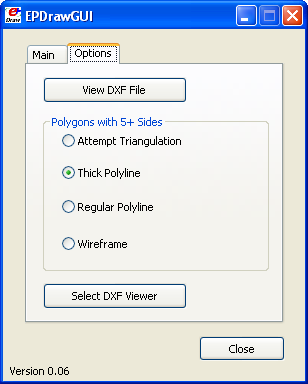
\includegraphics[width=0.9\textwidth, height=0.9\textheight, keepaspectratio=true]{media/image029.png}
\caption{EPDrawGUI Options Tab \protect \label{fig:epdrawgui-options-tab}}
\end{figure}
